%Préambule du document :
\documentclass[12pt, a4paper]{book}
%\usepackage[latin1]{inputenc} 
\usepackage[utf8]{inputenc} % accents
\usepackage{gensymb} % degree symbol ° (\degree)
\usepackage[T1]{fontenc} % | "`pipe"' character
\usepackage{graphicx}
\usepackage{titling}
\usepackage{amssymb} 
\usepackage{minitoc} % chapter's tocs
\usepackage{authblk} % author affiliations
\usepackage{fancyhdr} % modify the headers
\usepackage{tabularx} % tables not larger than A4
\usepackage[table]{xcolor} %colors inside the tables
\usepackage{float}
\usepackage{multicol} % multiple columns in some sections
\usepackage[inner=2cm,outer=2cm]{geometry} %A4 margins
\usepackage{siunitx}
\usepackage[labelfont=bf, margin=0.5cm]{caption} % for figure captions in minipages
\usepackage{hyperref} %link references (toc, citations) inside document
\usepackage{natbib} % to cite with parentheses and plain text et only year if you please...
\usepackage{amsmath}
 \usepackage{fixltx2e} % allows overrightarrow to be in caption
 \MakeRobust{\overrightarrow}




\bibliographystyle{plainnat} % reference style
\renewcommand{\bibname}{References} %Rename "`bibliography"' => "`references"'

\hypersetup{
    colorlinks,
    citecolor=brown,
    filecolor=green,
    linkcolor=red,
    urlcolor=blue
}
\hypersetup{linktocpage}


\pagestyle{fancy}
\fancyhead{}
\fancyfoot{}
\fancyhead[RO,LE]{\thepage}
\fancyhead[LO]{\leftmark}
\fancyhead[RE]{\rightmark}
\setcounter{tocdepth}{1} % we only want chapters and sections in toc
\setcounter{minitocdepth}{2} %we want sections and subsections in chapters' minitocs

\pretitle{%
  \begin{center}
  
  
\includegraphics[width=17cm]{../Logo_software.png}\\[\bigskipamount]
}
\posttitle{
\\
  \includegraphics[width=6.5cm]{tutorial04.png}\\[\bigskipamount]
\end{center}}

%\postdate{
%
\includegraphics[width=15cm]{logo_affiliations.png}
%}

\title{Tutorial 04: working with tags}



%\titlepicture[width=13cm]{Logo_software.png}
\author{Renaud LEBRUN}
\affil{Institut des Sciences de l'Evolution, Université de Montpellier, France}
\date{\today} 

\def\chaptername{Tutorial}
\setcounter{chapter}{4}
%Corps du document :
\begin{document}

\dominitoc	

\maketitle

\faketableofcontents

\addstarredchapter{Working with tags}

\markboth{Tutorial 04: Working with tags}{}

\minitoc 
Tutorial 04 includes:
\begin{itemize}
\item One .ntw (MorphoDig project) file
\item One .vtk surface file representing a right inner ear of \textit{Galago sp}
\item One .pos (position) file 
\item One .ori (orientation helper labels) file 
\item One .tgp (tag map) file
\item The present .pdf document
\end{itemize}





\section{About the specimen}

%\addcontentsline{toc}{section}{About the specimen}
The surface file enclosed in this tutorial represent three-dimensional reconstruction of the right inner ear of a strepsirrhine primate (\textit{Galago sp}) obtained by computerized microtomography at the MRI \si{\micro} CT.\\
Before using this tutorial, please download and read MorphoDig User Guide.


\section{A brief overview of enclosed files}
		Download and unzip the files associated to this tutorial. Open MorphoDig.
\subsection{Galago sp inner ear surface and position files}
	You may open the enclosed .vtk surface file (File -> Surface -> Open Surface, then select "Galago\_sp\_right\_ear.vtk", or drag and drop this file in the 3D main window). When opened
this way, the corresponding opened surface object is drawn grey, which indicates that this surface
is selected. You may interact with selected objects in different ways (see MorphoDig user guide for
further explanations).\\


By default (\includegraphics[scale=0.7]{../images/06/camera/move_cam2.png}), the camera rotates around the center of mass of all opened objects. This behavior is useful when the center of mass of an object (or of several ones) is far from the origin of the coordinate system. But by pressing the camera button (\includegraphics[scale=0.7]{../images/06/camera/move_cam2.png} -> 
\includegraphics[scale=0.7]{../images/06/camera/move_cam.png}), the camera will revolve around the center of the coordinate system (x=0, y=0, z=0).  The display grid is drawn using different colors depending on the camera rotation center (see Fig. \ref{grid_color} p.\pageref{grid_color}).



 As a general rule, when opening a new surface, it is strongly advised to change its position in order that it matches the 6 predefined camera positions :\\

\includegraphics[scale=0.7]{../images/06/camera/camera_right.png} view object from right side \\

\includegraphics[scale=0.7]{../images/06/camera/camera_left.png} view object from left side\\

\includegraphics[scale=0.7]{../images/06/camera/camera_front.png} view object from front side (default camera position)\\

\includegraphics[scale=0.7]{../images/06/camera/camera_back.png} view object from back side\\

\includegraphics[scale=0.7]{../images/06/camera/camera_above.png} view object from above\\

\includegraphics[scale=0.7]{../images/06/camera/camera_below.png} view object from below\\

In "object interaction mode(
\includegraphics[scale=0.7]{../images/04/move_mode.png})", selected objects can be translated and rotated using the left adn middle mouse buttons (in landmark 
\includegraphics[scale=0.7]{../images/04/Landmarks2.png} and camera  
\includegraphics[scale=0.7]{../images/04/camera_mode.png} selection modes, you also need to maintain ``CTRL" button pressed while dragging the left mouse button to achieve rotation and translation of selected objects). Alternatively, you may also use the "yellow sliders" located on the right side of the 3D main window to accomplish rotation and translation of selected objects. Rotation is achieved around the global center of mass of all currently selected objects.\\
\begin{figure}
  \centering
  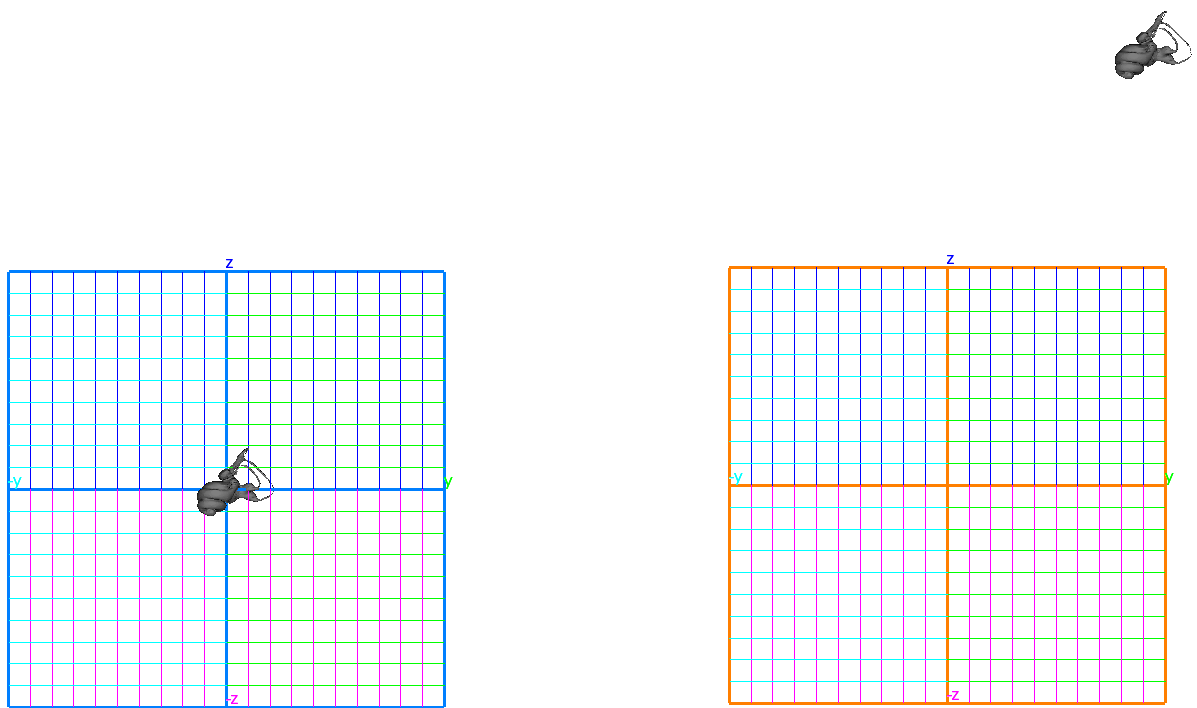
\includegraphics[scale=0.3]{grid.png} 
	\caption{Grid display color.  Left: when the camera revolves around the center of mass of all opened objects, the grid has a blue outline. Right: when the camera revolves around the origin of the coordinate system (x=0, y=0, z=0), the grid outline is displayed in orange.}
\label{grid_color}
 
\end{figure}

A convenient way to orient a right inner ear in a biologically relevant way is done as follows (see Fig. \ref{orientation} p.\pageref{orientation}):\\
1) place camera to view object from the front side (
\includegraphics[scale=0.7]{../images/06/camera/camera_front.png})\\
2) place the lateral semi-circular canal in the horizontal plane (x-y plane)\\
3) place camera  to view object from above ( 
\includegraphics[scale=0.7]{../images/06/camera/camera_above.png} )\\
4) rotate the inner around the z axis ("rz" yellow slider) until the later semicircular points towards the top left-hand part of the screen, and the cochlea points towards the bottom right-hand of the screen.\\
That way, when viewing the inner ear from the front side (
\includegraphics[scale=0.7]{../images/06/camera/camera_front.png}), it is approximately oriented in the same way as it would be within the cranium viewed from the front side as well.\\

The present tutorial contains a .pos (position) file, which you may open in order to place correctly the right ear of the \textit{Galago sp} (File -> Position-> Open Position for selected surfaces, then choose "Galago\_sp\_right\_ear.pos", see Fig. \ref{orientation} p.\pageref{orientation}).\\
All opened surfaces can be unselected by pressing "CTRL +D", or selected by pressing "CTRL +A". All selected objects can be deleted by pressing "Del".

\begin{figure}
  \centering
  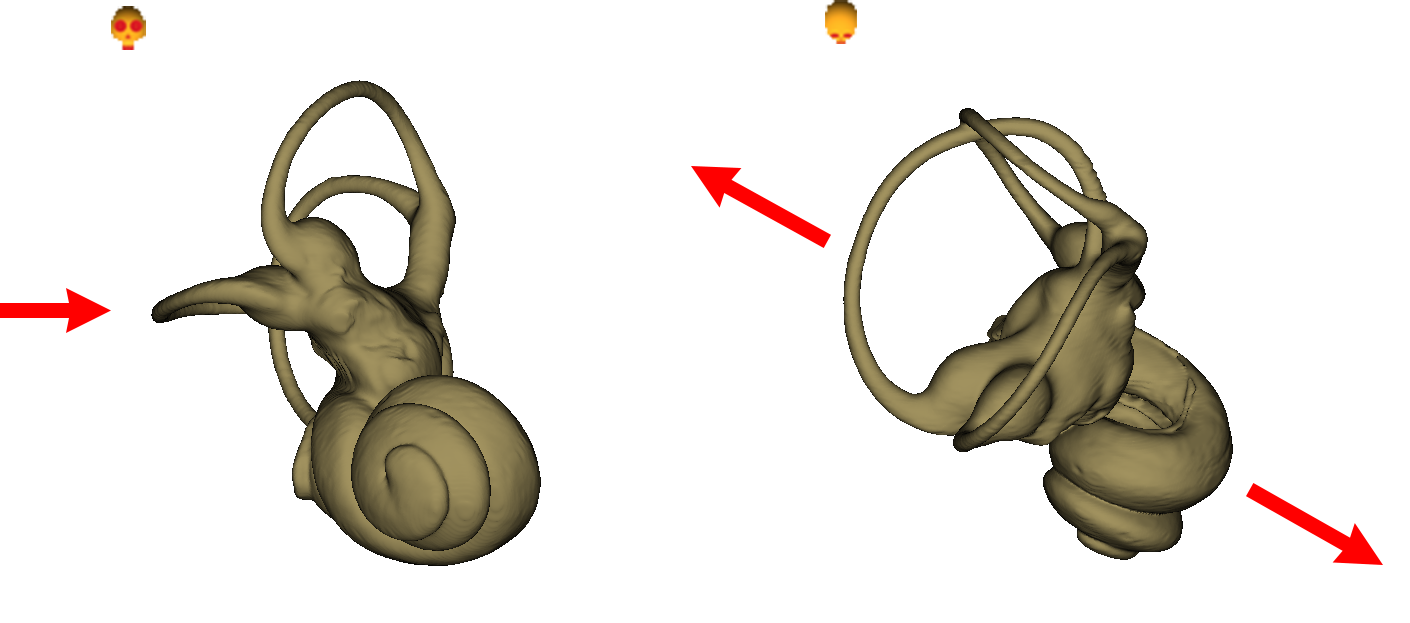
\includegraphics[scale=0.3]{pos.png} 
	\caption{A convenient way to orientate right inner ears.  Left: when viewed from the front side, the lateral canal is placed horizontally. Right: when viewed from above, the cochlea points towards the bottom right-hand of the screen, and the lateral canal towards the top left-hand of the screen.}
\label{orientation}
 
\end{figure}

\subsection{Galago sp tag map file}

All vertices of different biological structures can be given a specific integer values (0, 1, 2, 3 ...), in order to identify them. Such integer arrays are referred to as "tag arrays". A given unselected surface can be colored using the currently active tag array (identified by its "name"), if that surface contains a tag array of that name. To do so, the array display mode button must be pressed (
\includegraphics[scale=0.7]{../images/04/show_color_scale.png}), and a \textbf{tag} array must be selected as the currently active array (ex:
\includegraphics[scale=0.5]{../images/04/scalarcombo_tag.png}). The way tag arrays are translated into colors can be set up using tag maps, also referred to as "Lookup tables" (LUT) or color transfer functions. Such a LUT is enclosed within the tag map file ( "Galago\_sp\_right\_ear.tgp"). Open this file ("File->Tag maps->Import tag map", or drag and drop this file directly in the 3D main window). Then open the tags window ("File->Tags->Open Tags window", or click on "
\includegraphics[scale=0.7]{../images/04/tag_edit.png}". The Tag window should open (see Fig. \ref{tags_window} p.\pageref{tags_window}), and should contain the tag names and associated colors defined in "Galago\_sp\_right\_ear.tgp". See MorphoDig user guide for further explanation regarding the Tags window.\\

\begin{figure}
  \centering
  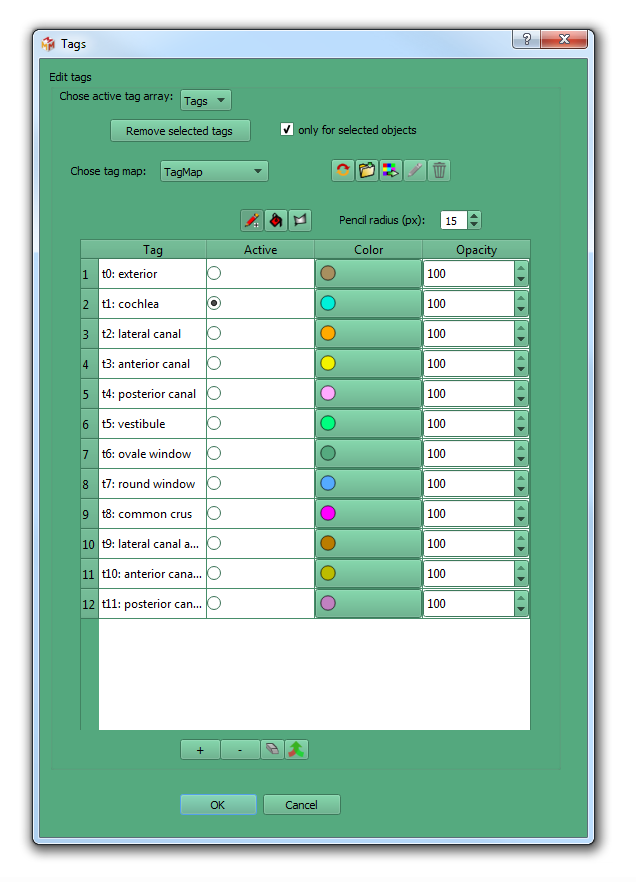
\includegraphics[scale=0.5]{tags_window.png}
\caption{Tags window.}	
\label{tags_window}
 \end{figure}


\subsection{Galago sp inner ear project file}
The present tutorial contains a project .ntw file, which may be useful to directly open the right inner ear
 in a convenient position, to make it transparent and to give it a color. First, delete all currently opened objects
(press "CTRL+A", then press "Del"). Then open the enclosed .ntw file (File -> Open Project, then select
"Galago\_sp\_right\_ear.ntw"). Once loaded, the right inner ear surface is opened, is given the position
enclosed in the "Galago\_sp\_right\_ear.pos" file, a color and a transparency. Note that the newly opened
surface is unselected. The surface file already contains a Tag array (named "Tags"), and you may set it as the currently active array.\\



\subsection{Galago sp inner ear .ori file}
The present tutorial contains a .ori file, which contains orientation labels for the coordinate system
orientation helper. You can load this file the enclosed .ori file ("File->Orientation helper labels -> Open Orientation labels", then select
"Galago\_sp\_right\_ear.ori"). Once loaded, the system coordinate orientation helper will show the following
labels :\\
+z axis : superior\\
-z axis : inferior\\
+y axis : medial\\
-y axis : lateral\\
+x axis : proximal\\
-x axis : distal\\
You may set your own orientation axis labels with the “Edit orientation labels” window (Edit-> Edit orientation labels)

\section{Tagging surfaces with MorphoDig}
Contrary to "scalar arrays" (see preceding section), tags are usually drawn manually with "painting tools". \\
For convenience purposes, as selected surfaces are drawn "grey" in MorphoDig, unselected surfaces objects can be tagged (tagging uniform "grey" objects without visual feedback would be uneasy). Tagging is the only way to modify an unselected surface in MorphoDig. \\
\subsection{Create a new empty tag array}\label{empty_tag_array}

\begin{minipage}{0.5\textwidth}
First, selecte the inner ear of \textit{Galago sp.} and click on "Tags->Create new empty tag array for each selected surface". Here, you may choose a name different from "Tags", as this array already exists. This option will create a new "empty" tag array. "Empty", in this context, means that all vertices are assigned to the "Exterior" tag (tag=0).\end{minipage} 
\begin{minipage}{0.5\textwidth}\centering
  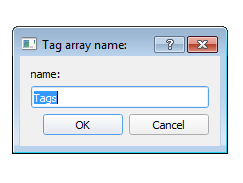
\includegraphics[scale=0.5]{../images/12/empty_tag_array.png}
 \captionof{figure}{Creating a new tag array}
 \end{minipage} 

Select the newly created tag array as the currently active array, and unselect the surface representing the inner ear of \textit{Galago sp.}


\subsection{Open the Tags window}
Click on "File->Tags->Open Tags window", or click on "
\includegraphics[scale=0.7]{../images/04/tag_edit.png}". The Tag window should open (see Fig. \ref{tags_window} p.\pageref{tags_window}). In this tutorial, you will use the pencil tag tool ("
\includegraphics[scale=0.7]{../images/12/pencil.png}") and the lasso tag tool ("
\includegraphics[scale=0.7]{../images/12/lasso.png}"). 

\subsection{Pencil tag tool.}
In the Tags window, click on "
\includegraphics[scale=0.7]{../images/12/pencil.png}".
You have two options:\\
 "T" pressed + left mouse click : tags the selected surface using currently active tag.\\
"T" pressed + right click : tags the selected surface using currently active tag \textbf{without color override}. Tag propagation will start at the picked vertex of a given color, but will stop when meeting another color different from that of "tag 0" (usually assigned to "Exterior").
\\Pencil tag size (in number of pixels) on the screen can be modified in the Tags window.





\subsection{Saving the project}
Saving a "project" makes it possible to save all opened selected objects and their properties (surface of the inner ear, its transparency, color and position, curve nodes, curve handles) altogether instead of one by one. 
To save all opened objects, do the following sequence of actions:\\
1) press "CTRL + A" to select all objects\\
2) click on "File->Project->Save Project" or on the button "save project" (
\includegraphics[scale=0.03]{../images/03/save_data.png})  inside the main window.\\
3) choose the desired options in the "Save Project" window (see Fig. \ref{save_project_file} p.\pageref{save_project_file} and the User Guide for further details regarding the available options)
\begin{figure}
  \centering  
 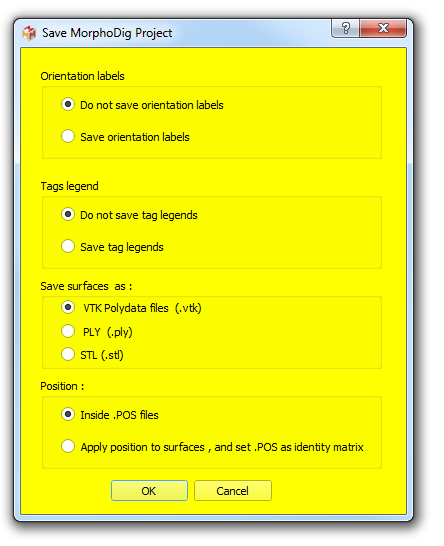
\includegraphics[scale=0.5]{../images/07/project/save_ntw.png}
 \captionof{figure}{Save project window.}
\label{save_project_file}
\end{figure}

The advantage of working with projects is that all involved objects and their properties (surfaces, landmarks, positions etc.) can be reloaded later all at once (and not 1 by 1). 

\section{Acknowledgements}
Thanks to the MRI imaging platform for the access to imaging facilities.

%\nocite{*}   % All bibliography items appear without citation in the text

%\cleardoublepage
%\phantomsection

%\addcontentsline{toc}{chapter}{References}
%  \bibliography{References/UsersGuide}		
\end{document} 

